% =============================================================================
% Projeto MATA60 - Banco de Dados (UFBA)
% Marco 1: Elaboração, Modelagem e Implantação do Banco de Dados
% =============================================================================

\documentclass[12pt,a4paper]{article}

\usepackage[utf8]{inputenc}
\usepackage[T1]{fontenc}
\usepackage[brazil]{babel}
\usepackage{times}
\usepackage[a4paper,margin=2.5cm]{geometry}
\usepackage{graphicx}
\usepackage{float}
\usepackage{caption}
\usepackage{subcaption}
\usepackage{array}
\usepackage{longtable}
\usepackage{booktabs}
\usepackage{multirow}
\usepackage{tabularx}
\usepackage{xcolor}
\usepackage{hyperref}
\usepackage{url}
\usepackage{listings}
\usepackage{amsmath,amssymb}
\usepackage{enumitem}
\usepackage{indentfirst}
\usepackage{setspace}
\usepackage{titlesec}
\usepackage{fancyhdr}

\hypersetup{
    colorlinks=true,
    linkcolor=black,
    citecolor=blue,
    urlcolor=blue,
    pdftitle={MATA60 - Sistema para Controle de Eventos Acadêmicos},
    pdfauthor={Deivid Costa, Douglas Aleixo, Igor Spinola, Pedro Larchert}
}

\definecolor{sqlkeyword}{rgb}{0.0, 0.0, 0.6}
\definecolor{sqlstring}{rgb}{0.6, 0.0, 0.0}
\definecolor{sqlcomment}{rgb}{0.25, 0.5, 0.35}
\definecolor{codebg}{rgb}{0.97,0.97,0.97}

\lstdefinelanguage{SQLext}{
  morekeywords={SELECT,FROM,WHERE,INSERT,INTO,VALUES,UPDATE,SET,DELETE,
    CREATE,TABLE,VIEW,INDEX,DROP,ALTER,ADD,PRIMARY,KEY,FOREIGN,REFERENCES,
    NOT,NULL,UNIQUE,CHECK,DEFAULT,JOIN,INNER,LEFT,RIGHT,FULL,OUTER,ON,
    GROUP,BY,ORDER,HAVING,UNION,INTERSECT,EXCEPT,AS,DISTINCT,COUNT,SUM,
    AVG,MIN,MAX,OVER,PARTITION,WINDOW,WITH,RECURSIVE,CASE,WHEN,THEN,ELSE,
    END,IN,EXISTS,BETWEEN,LIKE,AND,OR,IS,SERIAL,INTEGER,VARCHAR,TEXT,
    DATE,TIMESTAMP,BOOLEAN,NUMERIC,DECIMAL,EXPLAIN,ANALYZE,BEGIN,COMMIT,
    ROLLBACK,TRANSACTION,SCHEMA,CONSTRAINT,CASCADE,RESTRICT,USING,RETURNING,RANK},
  sensitive=false,
  morecomment=[l]{--},
  morecomment=[s]{/*}{*/},
  morestring=[b]'
}

\lstset{
    language=SQLext,
    basicstyle=\ttfamily\footnotesize,
    keywordstyle=\color{sqlkeyword}\bfseries,
    stringstyle=\color{sqlstring},
    commentstyle=\color{sqlcomment}\itshape,
    backgroundcolor=\color{codebg},
    frame=single,
    rulecolor=\color{black!30},
    breaklines=true,
    breakatwhitespace=true,
    showstringspaces=false,
    tabsize=2,
    captionpos=b,
    numbers=left,
    numberstyle=\tiny\color{gray},
    numbersep=8pt,
    xleftmargin=2em,
    framexleftmargin=1.5em
}

\onehalfspacing
\setlength{\parindent}{1.25cm}
\setlength{\parskip}{4pt}

\pagestyle{fancy}
\fancyhf{}
\fancyhead[L]{\small MATA60 -- Banco de Dados}
\fancyhead[R]{\small Marco 1 -- MIBD}
\fancyfoot[C]{\thepage}
\renewcommand{\headrulewidth}{0.4pt}

\titleformat{\section}{\normalfont\Large\bfseries}{\thesection.}{0.5em}{}
\titleformat{\subsection}{\normalfont\large\bfseries}{\thesubsection.}{0.5em}{}
\titleformat{\subsubsection}{\normalfont\normalsize\bfseries}{\thesubsubsection.}{0.5em}{}

% =============================================================================
\begin{document}

% ---------- Capa ----------
\begin{titlepage}
\begin{center}
    
\includegraphics[width=3cm]{Brasão_da_UFBA.png}\\[0.4cm]
    {\large \textbf{UNIVERSIDADE FEDERAL DA BAHIA}}\\
    {\large \textbf{INSTITUTO DE COMPUTAÇÃO}}\\
    {\large \textbf{MATA60 -- BANCO DE DADOS}}\\
    \vspace{0.5cm}
    {\normalsize Prof. Robespierre Pita}

    \vfill

    {\Large \textbf{Projeto da Disciplina -- Marco 1}}\\[0.5cm]
    {\LARGE \textbf{Elaboração, Modelagem e Implantação\\ do Banco de Dados}}\\[0.5cm]
    {\Large \emph{Estudo de Caso: Sistema para Controle de Eventos Acadêmicos}}

    \vfill

    {\large \textbf{Autores:}}\\[0.3cm]
    {\large Deivid Costa}\\
    {\large Douglas Aleixo}\\
    {\large Igor Spinola}\\
    {\large Pedro Larchert}\\

    \vfill

    {\large Salvador -- BA}\\
    {\large \today}
\end{center}
\end{titlepage}

\tableofcontents
\newpage

% =============================================================================
\begin{center}
    \textbf{\large Resumo}
\end{center}
\noindent
Este trabalho apresenta a modelagem e implantação de um banco de dados relacional
para gerenciamento de eventos acadêmicos, desenvolvido na disciplina MATA60 --
Banco de Dados da Universidade Federal da Bahia. O sistema cobre o ciclo completo
de um evento científico: inscrições com controle de pagamento, submissão e revisão
por pares de publicações, organização de anais e certificação de participantes.
O modelo foi construído com a notação de Peter Chen no BrModelo, traduzido para o
modelo relacional e implantado no PostgreSQL 16 via Docker. Foram elaboradas 10
consultas intermediárias envolvendo \texttt{JOIN}, \texttt{GROUP BY}, \texttt{COUNT}
e funções de janela (\texttt{WINDOW}).

\vspace{0.5cm}
\noindent\textbf{Palavras-chave:} Banco de Dados; PostgreSQL; Modelo Entidade-Relacionamento;
Eventos Acadêmicos; Revisão por Pares.

\newpage

% =============================================================================
\section{Introdução}
\label{sec:introducao}

Eventos científicos e acadêmicos -- como simpósios, conferências e workshops --
demandam uma infraestrutura de informação capaz de coordenar múltiplos atores e
processos simultâneos: organizadores, autores, revisores e participantes interagem
em torno de submissões, avaliações, inscrições e pagamentos. A ausência de um
sistema de dados bem estruturado torna esse processo suscetível a inconsistências,
perda de informação e dificuldades na prestação de contas.

Este projeto propõe um banco de dados relacional para cobrir esse domínio de forma
completa. Partindo do estudo de caso fornecido pelo professor, o grupo modelou,
implementou e populou o banco no PostgreSQL 16, elaborando também consultas
analíticas que respondem a perguntas reais de gestão de eventos.

As seções seguintes descrevem o estudo de caso e os requisitos levantados
(Seção~\ref{sec:descritivo}), a modelagem conceitual e lógica (Seção~\ref{sec:modelagem}),
a implantação do DDL (Seção~\ref{sec:implantacao}), as consultas elaboradas
(Seção~\ref{sec:consultas}) e as considerações finais
(Seção~\ref{sec:conclusao}).

% =============================================================================
\section{Descritivo do Projeto}
\label{sec:descritivo}

\subsection{Estudo de Caso Original}
\label{subsec:caso-original}

O estudo de caso atribuído pelo professor define um \textbf{Sistema para Controle
de Eventos Acadêmicos}. A motivação parte da necessidade de gestão eficiente de
submissões, revisões e inscrições em eventos científicos. Os requisitos originais
são:

\begin{enumerate}
    \item Gerenciar submissões de artigos e resumos.
    \item Acompanhar o processo de revisão por pares.
    \item Emitir certificados de participação.
    \item Permitir inscrições e pagamentos online.
    \item Organizar a programação dos eventos.
    \item Controlar a emissão de anais e proceedings.
\end{enumerate}

As tabelas principais sugeridas foram: Evento, Participante, Artigo, Revisor,
Inscrição, Pagamento e Certificado.

\subsection{Extensão Proposta ao Estudo de Caso}
\label{subsec:caso-estendido}

O grupo identificou algumas lacunas no estudo de caso original e propôs as
seguintes extensões:

\begin{itemize}
    \item \textbf{Tipos de publicação:} a distinção entre \emph{artigo completo}
    e \emph{resumo} foi representada como entidade própria (\texttt{tb\_tipo\_publicacao}),
    permitindo consultas analíticas sobre o perfil de cada evento.

    \item \textbf{Status de pagamento desacoplado:} o estado financeiro da inscrição
    foi separado em uma tabela de domínio (\texttt{tb\_status\_pagamento}) com valores
    CONCLUIDO, PENDENTE e CANCELADO, facilitando filtros e relatórios sem uso de
    \emph{magic numbers}.

    \item \textbf{Autoria múltipla:} o relacionamento N:M entre participantes e
    publicações (\texttt{rl\_autoria}) permite registrar coautoria e identificar
    participantes-pesquisadores ativos.

    \item \textbf{Revisão com resultado:} a tabela \texttt{rl\_revisao} armazena o
    parecer do revisor (\texttt{st\_aprovado}) e a data da revisão, possibilitando
    auditoria do processo de avaliação por pares.

    \item \textbf{Anais como relacionamento:} a associação entre evento e publicação
    nos anais foi modelada como tabela própria (\texttt{rl\_anais}), distinguindo
    publicações submetidas de publicações efetivamente aceitas e publicadas.
\end{itemize}

\subsection{Requisitos do Sistema}
\label{subsec:requisitos}

\subsubsection{Requisitos Funcionais (RF)}
\begin{description}[leftmargin=2.5cm,style=nextline]
    \item[\textbf{RF01}] O sistema deve permitir o cadastro de eventos com nome, local, datas de início e fim, preço e número de vagas.
    \item[\textbf{RF02}] O sistema deve permitir o cadastro de participantes com nome, CPF e e-mail únicos.
    \item[\textbf{RF03}] O sistema deve registrar inscrições de participantes em eventos, associadas a um método e status de pagamento.
    \item[\textbf{RF04}] O sistema deve permitir a submissão de publicações (artigos ou resumos) por participantes.
    \item[\textbf{RF05}] O sistema deve registrar a autoria de publicações, suportando múltiplos coautores.
    \item[\textbf{RF06}] O sistema deve gerenciar o processo de revisão por pares, associando revisores a publicações e registrando o parecer.
    \item[\textbf{RF07}] O sistema deve controlar quais publicações aprovadas compõem os anais de cada evento.
    \item[\textbf{RF08}] O sistema deve permitir a consulta da carga de revisão por revisor.
    \item[\textbf{RF09}] O sistema deve fornecer relatórios financeiros por evento e por método de pagamento.
    \item[\textbf{RF10}] O sistema deve distinguir publicações aprovadas das efetivamente apresentadas no evento.
\end{description}

\subsubsection{Requisitos Não-Funcionais (RNF)}
\begin{description}[leftmargin=2.5cm,style=nextline]
    \item[\textbf{RNF01}] Integridade referencial garantida via chaves estrangeiras declaradas no DDL.
    \item[\textbf{RNF02}] Unicidade de CPF e e-mail de participantes e revisores garantida por constraints \texttt{UNIQUE}.
    \item[\textbf{RNF03}] Nomenclatura de tabelas e colunas em português, seguindo prefixos de domínio (\texttt{tb\_} para entidades, \texttt{rl\_} para relacionamentos).
    \item[\textbf{RNF04}] O banco deve ser executável via Docker com inicialização automática do DDL e dos dados.
\end{description}

\subsection{Delimitação do Minimundo}
\label{subsec:minimundo}

O sistema modela o ciclo de vida de um evento acadêmico desde a abertura de
inscrições até a publicação dos anais. Estão no escopo: eventos, participantes,
inscrições, publicações, autoria, revisão e anais. Estão fora do escopo:
emissão de certificados, programação detalhada das sessões e integração com
gateways de pagamento externos.

\begin{table}[H]
\centering
\caption{Mapeamento entre elementos do minimundo e requisitos.}
\label{tab:minimundo-requisitos}
\small
\begin{tabularx}{\textwidth}{|l|X|l|}
\hline
\textbf{Elemento} & \textbf{Descrição} & \textbf{RF} \\
\hline
\texttt{tb\_evento}            & Dados do evento: nome, local, datas, preço, vagas        & RF01 \\
\hline
\texttt{tb\_participante}      & Cadastro de pessoas: nome, CPF, e-mail                   & RF02 \\
\hline
\texttt{rl\_inscricao}         & Vínculo participante-evento com pagamento                & RF03 \\
\hline
\texttt{tb\_status\_pagamento} & Domínio: CONCLUIDO, PENDENTE, CANCELADO                  & RF03, RF09 \\
\hline
\texttt{tb\_publicacao}        & Submissões com título, conteúdo, aprovação e apresentação & RF04, RF10 \\
\hline
\texttt{tb\_tipo\_publicacao}  & Domínio: Artigo, Resumo                                  & RF04 \\
\hline
\texttt{rl\_autoria}           & Relação N:M participante-publicação                      & RF05 \\
\hline
\texttt{tb\_revisor}           & Cadastro de avaliadores                                  & RF06 \\
\hline
\texttt{rl\_revisao}           & Parecer do revisor com data e resultado                  & RF06, RF08 \\
\hline
\texttt{rl\_anais}             & Publicações aceitas vinculadas ao evento                 & RF07 \\
\hline
\end{tabularx}
\end{table}

% =============================================================================
\section{Modelagem}
\label{sec:modelagem}

\subsection{Modelo Conceitual (MER)}
\label{subsec:mer}

\begin{figure}[H]
    \centering
    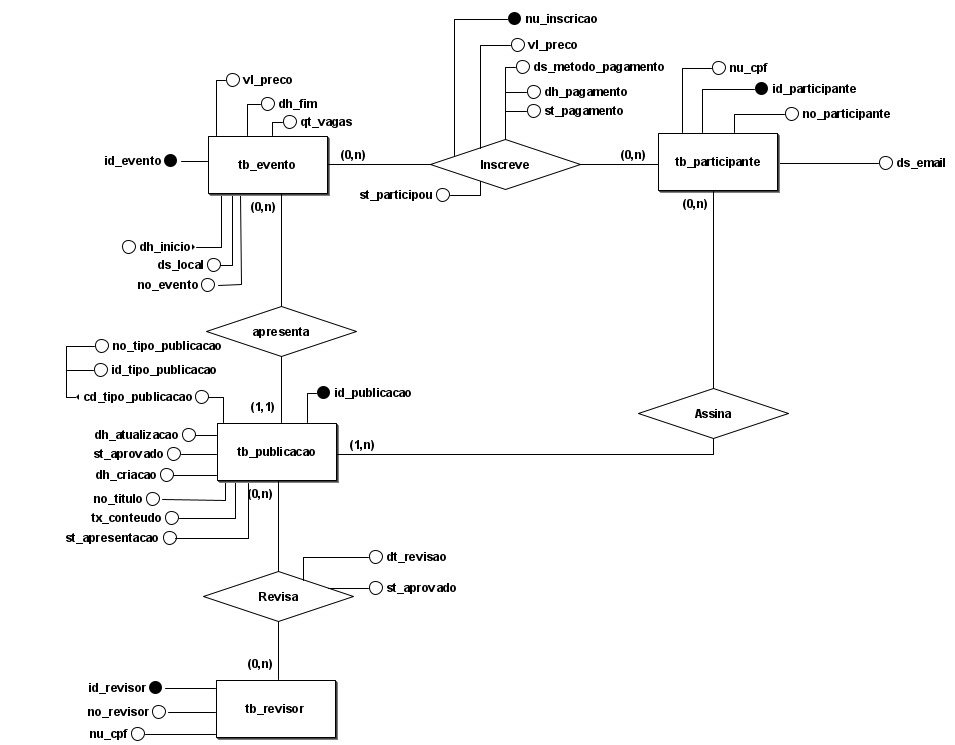
\includegraphics[width=0.95\textwidth]{BRMODELO_SQL.jpeg}
    \caption{Modelo Entidade-Relacionamento elaborado no BrModelo.}
    \label{fig:mer}
\end{figure}

A Figura~\ref{fig:mer} apresenta o modelo conceitual. As entidades principais
são \texttt{Evento}, \texttt{Participante}, \texttt{Publicacao} e \texttt{Revisor}.
Os relacionamentos N:M (\emph{autoria}, \emph{revisão}, \emph{inscrição} e
\emph{anais}) foram representados como tabelas associativas no modelo lógico.

\subsection{Modelo Lógico}
\label{subsec:logico}

\begin{figure}[H]
    \centering
    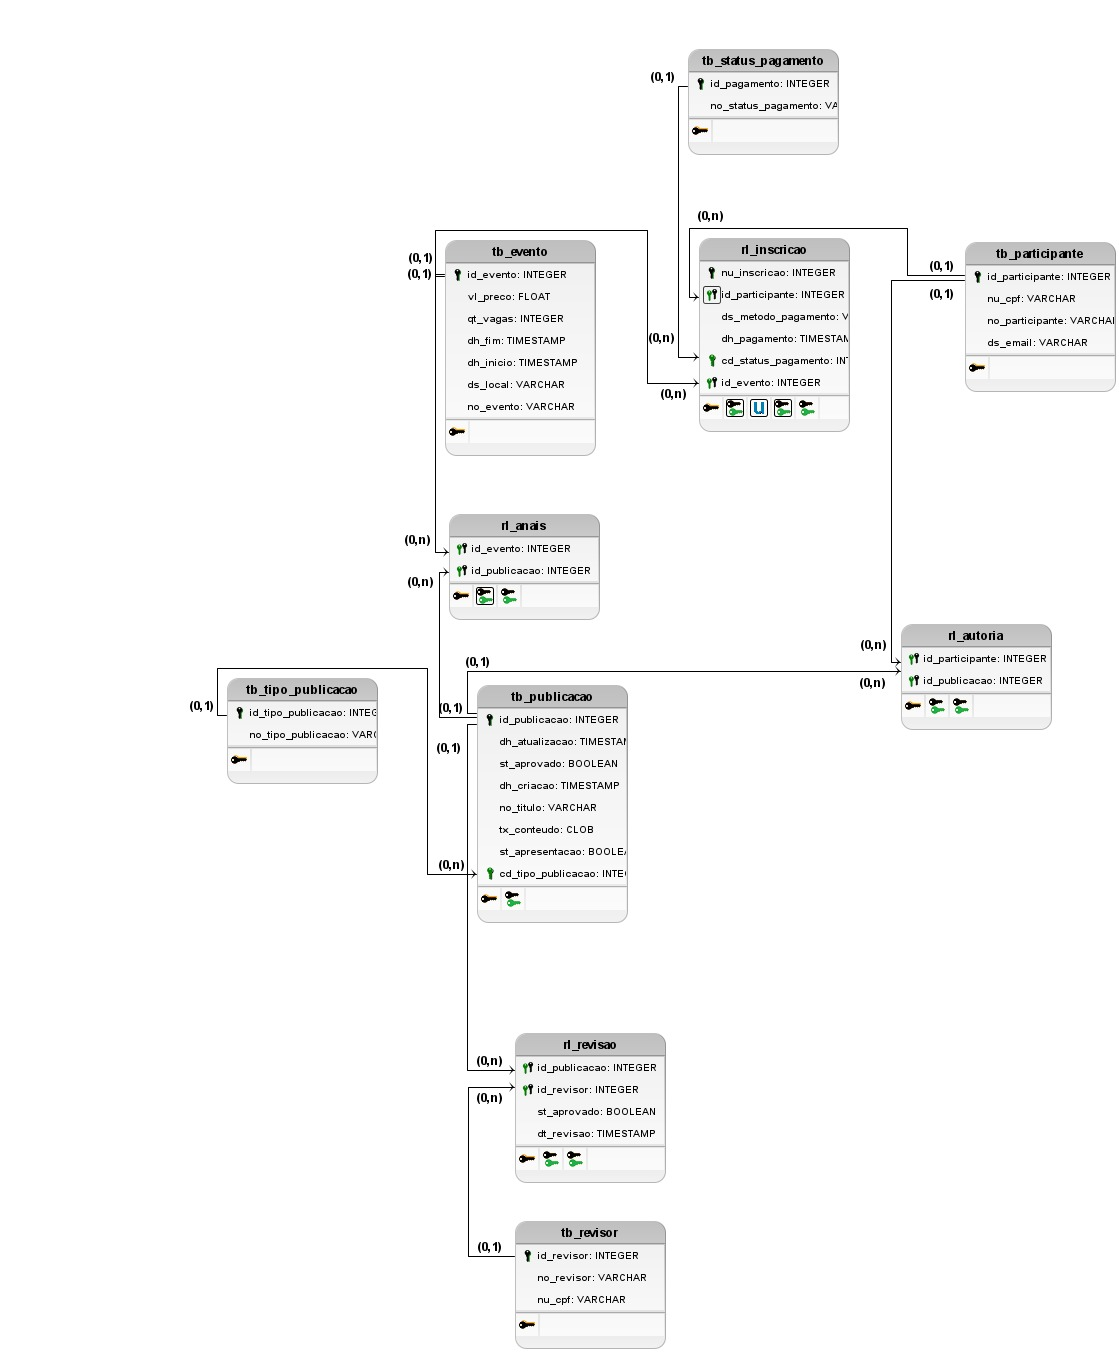
\includegraphics[width=0.95\textwidth]{MODELO_LOGICO.jpeg}
    \caption{Modelo lógico relacional.}
    \label{fig:logico}
\end{figure}

O modelo lógico resultante, apresentado na Figura~\ref{fig:logico}, é composto
por 10 tabelas. A notação textual do esquema é:

\begin{lstlisting}[caption={Esquema lógico relacional.}, label={lst:logico}, language={}]
tb_evento(id_evento PK, no_evento, ds_local, dh_inicio, dh_fim, vl_preco, qt_vagas)
tb_participante(id_participante PK, no_participante, nu_cpf UNIQUE, ds_email UNIQUE)
tb_revisor(id_revisor PK, no_revisor, nu_cpf UNIQUE)
tb_publicacao(id_publicacao PK, no_titulo, tx_conteudo, dh_criacao, dh_atualizacao,
              st_aprovado, st_apresentacao, cd_tipo_publicacao FK)
tb_tipo_publicacao(id_tipo_publicacao PK, no_tipo_publicacao UNIQUE)
tb_status_pagamento(id_pagamento PK, no_status_pagamento UNIQUE)
rl_inscricao(nu_inscricao, id_participante FK, id_evento FK, cd_status_pagamento FK,
             ds_metodo_pagamento, dh_pagamento, PK(nu_inscricao, id_participante, id_evento))
rl_autoria(id_participante FK, id_publicacao FK, PK(id_participante, id_publicacao))
rl_revisao(id_publicacao FK, id_revisor FK, st_aprovado, dt_revisao,
           PK(id_publicacao, id_revisor))
rl_anais(id_evento FK, id_publicacao FK, PK(id_evento, id_publicacao))
\end{lstlisting}

\subsection{Convenções de Nomenclatura}
\label{subsec:nomenclatura}

A nomenclatura segue as diretrizes do MAD/DATASUS e da ISO/IEC 11179-5:
prefixo \texttt{tb\_} para entidades, \texttt{rl\_} para relacionamentos N:M;
colunas nomeadas com prefixo semântico (\texttt{id\_} para identificadores,
\texttt{no\_} para nomes, \texttt{ds\_} para descrições, \texttt{dh\_} para
data/hora, \texttt{st\_} para booleanos de estado, \texttt{cd\_} para
códigos de referência, \texttt{vl\_} para valores monetários e \texttt{qt\_}
para quantidades).

% =============================================================================
\section{Implantação}
\label{sec:implantacao}

\subsection{Script DDL}
\label{subsec:ddl}

O banco foi implantado no PostgreSQL 16. O script DDL cria as tabelas com suas
restrições e, em seguida, declara todas as chaves estrangeiras via
\texttt{ALTER TABLE}.

\begin{lstlisting}[caption={DDL -- tabelas de domínio e entidades principais.}, label={lst:ddl1}]
CREATE TABLE tb_status_pagamento (
    id_pagamento INTEGER PRIMARY KEY,
    no_status_pagamento VARCHAR(30) UNIQUE NOT NULL
);

CREATE TABLE tb_tipo_publicacao (
    id_tipo_publicacao INTEGER PRIMARY KEY,
    no_tipo_publicacao VARCHAR(50) UNIQUE NOT NULL
);

CREATE TABLE tb_evento (
    id_evento INTEGER PRIMARY KEY,
    no_evento VARCHAR(100) NOT NULL,
    ds_local VARCHAR(200) NOT NULL,
    dh_inicio TIMESTAMP NOT NULL,
    dh_fim TIMESTAMP NOT NULL,
    vl_preco DECIMAL(10,2) NOT NULL,
    qt_vagas INTEGER NOT NULL
);

CREATE TABLE tb_participante (
    id_participante INTEGER PRIMARY KEY,
    no_participante VARCHAR(100) NOT NULL,
    nu_cpf VARCHAR(11) UNIQUE NOT NULL,
    ds_email VARCHAR(150) UNIQUE NOT NULL
);

CREATE TABLE tb_revisor (
    id_revisor INTEGER PRIMARY KEY,
    no_revisor VARCHAR(100) NOT NULL,
    nu_cpf VARCHAR(11) UNIQUE NOT NULL
);

CREATE TABLE tb_publicacao (
    id_publicacao INTEGER PRIMARY KEY,
    no_titulo VARCHAR(200) NOT NULL,
    tx_conteudo TEXT NOT NULL,
    dh_criacao TIMESTAMP NOT NULL,
    dh_atualizacao TIMESTAMP,
    st_aprovado BOOLEAN NOT NULL,
    st_apresentacao BOOLEAN NOT NULL,
    cd_tipo_publicacao INTEGER NOT NULL
);
\end{lstlisting}

\begin{lstlisting}[caption={DDL -- tabelas associativas (relacionamentos N:M).}, label={lst:ddl2}]
CREATE TABLE rl_inscricao (
    nu_inscricao INTEGER UNIQUE NOT NULL,
    id_participante INTEGER NOT NULL,
    id_evento INTEGER NOT NULL,
    cd_status_pagamento INTEGER NOT NULL,
    ds_metodo_pagamento VARCHAR(50) NOT NULL,
    dh_pagamento TIMESTAMP,
    PRIMARY KEY (nu_inscricao, id_participante, id_evento)
);

CREATE TABLE rl_autoria (
    id_participante INTEGER NOT NULL,
    id_publicacao INTEGER NOT NULL,
    PRIMARY KEY (id_participante, id_publicacao)
);

CREATE TABLE rl_revisao (
    id_publicacao INTEGER NOT NULL,
    id_revisor INTEGER NOT NULL,
    st_aprovado BOOLEAN NOT NULL,
    dt_revisao DATE NOT NULL,
    PRIMARY KEY (id_publicacao, id_revisor)
);

CREATE TABLE rl_anais (
    id_evento INTEGER NOT NULL,
    id_publicacao INTEGER NOT NULL,
    PRIMARY KEY (id_evento, id_publicacao)
);
\end{lstlisting}

\begin{lstlisting}[caption={DDL -- declaração das chaves estrangeiras.}, label={lst:ddl3}]
ALTER TABLE tb_publicacao
    ADD CONSTRAINT FK_tb_publicacao_tipo_publicacao
    FOREIGN KEY (cd_tipo_publicacao) REFERENCES tb_tipo_publicacao (id_tipo_publicacao);

ALTER TABLE rl_inscricao
    ADD CONSTRAINT FK_rl_inscricao_id_evento
    FOREIGN KEY (id_evento) REFERENCES tb_evento (id_evento);

ALTER TABLE rl_inscricao
    ADD CONSTRAINT FK_rl_inscricao_id_participante
    FOREIGN KEY (id_participante) REFERENCES tb_participante (id_participante);

ALTER TABLE rl_inscricao
    ADD CONSTRAINT FK_rl_inscricao_status_pagamento
    FOREIGN KEY (cd_status_pagamento) REFERENCES tb_status_pagamento (id_pagamento);

ALTER TABLE rl_anais
    ADD CONSTRAINT FK_rl_anais_id_evento
    FOREIGN KEY (id_evento) REFERENCES tb_evento (id_evento);

ALTER TABLE rl_anais
    ADD CONSTRAINT FK_rl_anais_id_publicacao
    FOREIGN KEY (id_publicacao) REFERENCES tb_publicacao (id_publicacao);

ALTER TABLE rl_autoria
    ADD CONSTRAINT FK_rl_autoria_participante
    FOREIGN KEY (id_participante) REFERENCES tb_participante (id_participante);

ALTER TABLE rl_autoria
    ADD CONSTRAINT FK_rl_autoria_publicacao
    FOREIGN KEY (id_publicacao) REFERENCES tb_publicacao (id_publicacao);

ALTER TABLE rl_revisao
    ADD CONSTRAINT FK_rl_revisao_publicacao
    FOREIGN KEY (id_publicacao) REFERENCES tb_publicacao (id_publicacao);

ALTER TABLE rl_revisao
    ADD CONSTRAINT FK_rl_revisao_revisao
    FOREIGN KEY (id_revisor) REFERENCES tb_revisor (id_revisor);
\end{lstlisting}

\subsection{Ambiente de Execução}
\label{subsec:docker}

O banco foi containerizado com Docker Compose. Ao executar \texttt{docker compose up},
o PostgreSQL 16 é iniciado e os scripts DDL e de inserção são aplicados automaticamente
via \texttt{/docker-entrypoint-initdb.d/}. Um serviço MySQL 8.0 também está disponível
para comparações.

% =============================================================================
\section{Consultas Intermediárias}
\label{sec:consultas}

As 10 consultas a seguir envolvem pelo menos 3 tabelas e utilizam duas ou mais
das funções \texttt{JOIN}, \texttt{GROUP BY}, \texttt{COUNT} e \texttt{WINDOW}.

% ------------------------------------------------------------------
\subsubsection*{QI01 -- Eventos com mais publicações nos anais}
\textbf{Requisitos atendidos:} RF07 \\
\textbf{Objetivo:} Rankear eventos pela quantidade de publicações que entraram nos anais.\\
\textbf{Recursos:} JOIN, GROUP BY, COUNT.
\begin{lstlisting}[caption={QI01 -- Eventos com mais publicações nos anais.}]
SELECT tb_evento.id_evento, tb_evento.no_evento,
       COUNT(id_publicacao) AS tot_publi
FROM rl_anais
    JOIN tb_evento ON tb_evento.id_evento = rl_anais.id_evento
GROUP BY tb_evento.id_evento, tb_evento.no_evento
ORDER BY tot_publi DESC;
\end{lstlisting}

% ------------------------------------------------------------------
\subsubsection*{QI02 -- Quantidade de coautores por publicação aprovada}
\textbf{Requisitos atendidos:} RF04, RF05 \\
\textbf{Objetivo:} Para cada publicação aprovada, mostrar título e número de autores.\\
\textbf{Recursos:} JOIN, WHERE, GROUP BY, COUNT.
\begin{lstlisting}[caption={QI02 -- Coautores por publicação aprovada.}]
SELECT rl_autoria.id_publicacao, no_titulo, COUNT(id_participante) AS qt_autores
FROM rl_autoria
    JOIN tb_publicacao ON tb_publicacao.id_publicacao = rl_autoria.id_publicacao
WHERE st_aprovado = TRUE
GROUP BY rl_autoria.id_publicacao, no_titulo
ORDER BY rl_autoria.id_publicacao ASC;
\end{lstlisting}

% ------------------------------------------------------------------
\subsubsection*{QI03 -- Participantes que também são autores}
\textbf{Requisitos atendidos:} RF02, RF05 \\
\textbf{Objetivo:} Listar participantes que publicaram pelo menos um artigo.\\
\textbf{Recursos:} JOIN, GROUP BY.
\begin{lstlisting}[caption={QI03 -- Participantes que também são autores.}]
SELECT tb_participante.id_participante, no_participante
FROM tb_participante
    JOIN rl_autoria ON rl_autoria.id_participante = tb_participante.id_participante
GROUP BY tb_participante.id_participante
ORDER BY tb_participante.id_participante;
\end{lstlisting}

% ------------------------------------------------------------------
\subsubsection*{QI04 -- Distribuição de status de pagamento por evento}
\textbf{Requisitos atendidos:} RF03, RF09 \\
\textbf{Objetivo:} Mostrar quantas inscrições estão em cada status (CONCLUIDO, PENDENTE, CANCELADO) por evento.\\
\textbf{Recursos:} JOIN, GROUP BY, COUNT.
\begin{lstlisting}[caption={QI04 -- Status de pagamento por evento.}]
SELECT rl_inscricao.id_evento, no_status_pagamento,
       COUNT(nu_inscricao) AS qt_inscricoes
FROM rl_inscricao
    JOIN tb_evento ON tb_evento.id_evento = rl_inscricao.id_evento
    JOIN tb_status_pagamento
        ON tb_status_pagamento.id_pagamento = rl_inscricao.cd_status_pagamento
GROUP BY rl_inscricao.id_evento, rl_inscricao.cd_status_pagamento, no_status_pagamento
ORDER BY rl_inscricao.id_evento ASC;
\end{lstlisting}

% ------------------------------------------------------------------
\subsubsection*{QI05 -- Publicações por tipo em cada evento}
\textbf{Requisitos atendidos:} RF04, RF07 \\
\textbf{Objetivo:} Contar quantos artigos e resumos cada evento publicou nos anais.\\
\textbf{Recursos:} INNER JOIN (4 tabelas), GROUP BY, COUNT.
\begin{lstlisting}[caption={QI05 -- Publicações por tipo em cada evento.}]
SELECT tb_evento.no_evento, tb_tipo_publicacao.no_tipo_publicacao,
       COUNT(*) AS total
FROM tb_evento
    INNER JOIN rl_anais ON tb_evento.id_evento = rl_anais.id_evento
    INNER JOIN tb_publicacao
        ON tb_publicacao.id_publicacao = rl_anais.id_publicacao
    INNER JOIN tb_tipo_publicacao
        ON tb_publicacao.cd_tipo_publicacao = tb_tipo_publicacao.id_tipo_publicacao
GROUP BY tb_evento.no_evento, tb_tipo_publicacao.no_tipo_publicacao
ORDER BY total DESC;
\end{lstlisting}

% ------------------------------------------------------------------
\subsubsection*{QI06 -- Eventos com 100\% das inscrições pagas}
\textbf{Requisitos atendidos:} RF03, RF09 \\
\textbf{Objetivo:} Listar eventos sem inadimplência (nenhuma inscrição PENDENTE ou CANCELADA).\\
\textbf{Recursos:} JOIN, subquery, WHERE.
\begin{lstlisting}[caption={QI06 -- Eventos com todas as inscrições CONCLUIDO.}]
SELECT DISTINCT tb_evento.id_evento, no_evento
FROM tb_evento
    JOIN (
        SELECT rl_inscricao.id_evento,
               COUNT(nu_inscricao) AS tot_sem_pagar
        FROM rl_inscricao
            JOIN tb_evento ON tb_evento.id_evento = rl_inscricao.id_evento
        WHERE cd_status_pagamento = 2 OR cd_status_pagamento = 3
        GROUP BY rl_inscricao.id_evento
    ) ta ON ta.id_evento = tb_evento.id_evento
WHERE ta.tot_sem_pagar < 1
ORDER BY tb_evento.id_evento ASC;
\end{lstlisting}

% ------------------------------------------------------------------
\subsubsection*{QI07 -- Carga de revisão por revisor}
\textbf{Requisitos atendidos:} RF06, RF08 \\
\textbf{Objetivo:} Mostrar quantas publicações cada revisor avaliou, ordenado por carga decrescente.\\
\textbf{Recursos:} JOIN, GROUP BY, COUNT.
\begin{lstlisting}[caption={QI07 -- Carga de revisão por revisor.}]
SELECT r.id_revisor, r.no_revisor,
       COUNT(rl.id_publicacao) AS qtd_publicacoes_revisadas
FROM tb_revisor r
    JOIN rl_revisao rl ON r.id_revisor = rl.id_revisor
GROUP BY r.id_revisor, r.no_revisor
ORDER BY qtd_publicacoes_revisadas DESC;
\end{lstlisting}

% ------------------------------------------------------------------
\subsubsection*{QI08 -- Publicações aprovadas e apresentadas por evento}
\textbf{Requisitos atendidos:} RF07, RF10 \\
\textbf{Objetivo:} Contar quantas publicações foram aprovadas e efetivamente apresentadas em cada evento.\\
\textbf{Recursos:} JOIN, WHERE, GROUP BY, COUNT.
\begin{lstlisting}[caption={QI08 -- Aprovadas e apresentadas por evento.}]
SELECT tb_evento.no_evento, COUNT(*) AS qt_apresentadas
FROM tb_evento
    JOIN rl_anais ON rl_anais.id_evento = tb_evento.id_evento
    JOIN tb_publicacao ON tb_publicacao.id_publicacao = rl_anais.id_publicacao
WHERE tb_publicacao.st_aprovado = TRUE
  AND tb_publicacao.st_apresentacao = TRUE
GROUP BY tb_evento.no_evento
ORDER BY tb_evento.no_evento ASC;
\end{lstlisting}

% ------------------------------------------------------------------
\subsubsection*{QI09 -- Receita por método de pagamento}
\textbf{Requisitos atendidos:} RF03, RF09 \\
\textbf{Objetivo:} Somar a receita confirmada (CONCLUIDO) por método (crédito, débito, pix) em cada evento.\\
\textbf{Recursos:} JOIN, WHERE, GROUP BY, SUM.
\begin{lstlisting}[caption={QI09 -- Receita por método de pagamento.}]
SELECT tb_evento.no_evento, rl_inscricao.ds_metodo_pagamento,
       COUNT(*) AS total_metodo,
       SUM(tb_evento.vl_preco) AS total_vendas
FROM tb_evento
    JOIN rl_inscricao ON rl_inscricao.id_evento = tb_evento.id_evento
    JOIN tb_status_pagamento
        ON tb_status_pagamento.id_pagamento = rl_inscricao.cd_status_pagamento
WHERE tb_status_pagamento.no_status_pagamento = 'CONCLUIDO'
GROUP BY tb_evento.no_evento, rl_inscricao.ds_metodo_pagamento
ORDER BY total_vendas DESC;
\end{lstlisting}

% ------------------------------------------------------------------
\subsubsection*{QI10 -- Ranking de eventos por receita (WINDOW)}
\textbf{Requisitos atendidos:} RF09 \\
\textbf{Objetivo:} Usar \texttt{RANK()} para posicionar cada evento pelo total de receita confirmada.\\
\textbf{Recursos:} JOIN, GROUP BY, SUM, WINDOW (RANK).
\begin{lstlisting}[caption={QI10 -- Ranking de receita com RANK().}]
SELECT no_evento, total_receita,
       RANK() OVER (ORDER BY total_receita DESC) AS posicao
FROM (
    SELECT tb_evento.no_evento,
           SUM(tb_evento.vl_preco) AS total_receita
    FROM tb_evento
        JOIN rl_inscricao ON rl_inscricao.id_evento = tb_evento.id_evento
        JOIN tb_status_pagamento
            ON tb_status_pagamento.id_pagamento = rl_inscricao.cd_status_pagamento
    WHERE tb_status_pagamento.no_status_pagamento = 'CONCLUIDO'
    GROUP BY tb_evento.no_evento
) ranking;
\end{lstlisting}

% ------------------------------------------------------------------
\subsection{Consultas Avançadas}
\label{subsec:consultas-adv}
% Regra: mínimo 3 tabelas + 3 das funções {SUB-CONSULTAS, JOIN, GROUP BY, WINDOW, COUNT}.
% São 20 consultas avançadas.

\subsubsection{Consulta Avançada 01 -- [Título]}
\textbf{Requisitos atendidos:} [...] \\
\textbf{Objetivo:} [...] \\
\textbf{Recursos utilizados:} [...].
\begin{lstlisting}[caption={Consulta Avançada 01.}]
-- A preencher
\end{lstlisting}

\subsubsection{Consulta Avançada 02 -- [Título]}
\subsubsection{Consulta Avançada 03 -- [Título]}
\subsubsection{Consulta Avançada 04 -- [Título]}
\subsubsection{Consulta Avançada 05 -- [Título]}
\subsubsection{Consulta Avançada 06 -- [Título]}
\subsubsection{Consulta Avançada 07 -- [Título]}
\subsubsection{Consulta Avançada 08 -- [Título]}
\subsubsection{Consulta Avançada 09 -- [Título]}
\subsubsection{Consulta Avançada 10 -- [Título]}
\subsubsection{Consulta Avançada 11 -- [Título]}
\subsubsection{Consulta Avançada 12 -- [Título]}
\subsubsection{Consulta Avançada 13 -- [Título]}
\subsubsection{Consulta Avançada 14 -- [Título]}
\subsubsection{Consulta Avançada 15 -- [Título]}
\subsubsection{Consulta Avançada 16 -- [Título]}
\subsubsection{Consulta Avançada 17 -- [Título]}
\subsubsection{Consulta Avançada 18 -- [Título]}
\subsubsection{Consulta Avançada 19 -- [Título]}
\subsubsection{Consulta Avançada 20 -- [Título]}

% ------------------------------------------------------------------
\subsection{Mapa Consulta $\times$ Requisito}

\begin{longtable}{|c|l|l|l|}
\caption{Associação entre consultas, requisitos atendidos e recursos SQL utilizados.}
\label{tab:consultas-req}\\
\hline
\textbf{ID} & \textbf{Tipo} & \textbf{Requisito} & \textbf{Recursos SQL} \\
\hline
\endfirsthead
\hline
\textbf{ID} & \textbf{Tipo} & \textbf{Requisito} & \textbf{Recursos SQL} \\
\hline
\endhead
QI01 & Intermediária & RF07 & JOIN, GROUP BY, COUNT \\
QI02 & Intermediária & RF04, RF05 & JOIN, WHERE, GROUP BY, COUNT \\
QI03 & Intermediária & RF02, RF05 & JOIN, GROUP BY \\
QI04 & Intermediária & RF03, RF09 & JOIN, GROUP BY, COUNT \\
QI05 & Intermediária & RF04, RF07 & INNER JOIN (4 tabelas), GROUP BY, COUNT \\
QI06 & Intermediária & RF03, RF09 & JOIN, subquery, WHERE \\
QI07 & Intermediária & RF06, RF08 & JOIN, GROUP BY, COUNT \\
QI08 & Intermediária & RF07, RF10 & JOIN, WHERE, GROUP BY, COUNT \\
QI09 & Intermediária & RF03, RF09 & JOIN, WHERE, GROUP BY, SUM \\
QI10 & Intermediária & RF09 & JOIN, GROUP BY, SUM, RANK() WINDOW \\
\hline
QA01 & Avançada & [RFXX] & SUB-QUERY, JOIN, GROUP BY \\
QA02 & Avançada & [RFXX] & [...] \\
QA03 & Avançada & [RFXX] & [...] \\
QA04 & Avançada & [RFXX] & [...] \\
QA05 & Avançada & [RFXX] & [...] \\
QA06 & Avançada & [RFXX] & [...] \\
QA07 & Avançada & [RFXX] & [...] \\
QA08 & Avançada & [RFXX] & [...] \\
QA09 & Avançada & [RFXX] & [...] \\
QA10 & Avançada & [RFXX] & [...] \\
QA11 & Avançada & [RFXX] & [...] \\
QA12 & Avançada & [RFXX] & [...] \\
QA13 & Avançada & [RFXX] & [...] \\
QA14 & Avançada & [RFXX] & [...] \\
QA15 & Avançada & [RFXX] & [...] \\
QA16 & Avançada & [RFXX] & [...] \\
QA17 & Avançada & [RFXX] & [...] \\
QA18 & Avançada & [RFXX] & [...] \\
QA19 & Avançada & [RFXX] & [...] \\
QA20 & Avançada & [RFXX] & [...] \\
\hline
\end{longtable}

% =============================================================================
\section{Plano de Indexação e Avaliação de Desempenho}
\label{sec:indexacao}

\subsection{Justificativa dos Índices Propostos}
\label{subsec:indices-justif}
[Apresentar e justificar os índices propostos a partir da análise das
consultas elaboradas. Considerar índices B-Tree, Hash, GIN/GiST conforme
o caso, sempre justificando teoricamente.]

\begin{table}[H]
\centering
\caption{Plano de indexação proposto.}
\label{tab:indices}
\small
\begin{tabularx}{\textwidth}{|l|l|l|X|}
\hline
\textbf{Índice} & \textbf{Tabela} & \textbf{Coluna(s) / Tipo} & \textbf{Consultas beneficiadas} \\
\hline
idx\_inscricao\_evento    & rl\_inscricao    & (id\_evento) -- B-Tree       & QI04, QI06, QI09, QI10 \\
idx\_inscricao\_status    & rl\_inscricao    & (cd\_status\_pagamento) -- B-Tree & QI04, QI06, QI09, QI10 \\
idx\_anais\_evento        & rl\_anais        & (id\_evento) -- B-Tree       & QI01, QI05, QI08 \\
idx\_autoria\_participante & rl\_autoria     & (id\_participante) -- B-Tree & QI02, QI03 \\
idx\_revisao\_revisor     & rl\_revisao      & (id\_revisor) -- B-Tree      & QI07 \\
idx\_publicacao\_aprovado & tb\_publicacao   & (st\_aprovado) -- B-Tree     & QI02, QI08 \\
\hline
\end{tabularx}
\end{table}

\begin{lstlisting}[caption={DDL dos índices.},label={lst:ddl-indices}]
CREATE INDEX idx_inscricao_evento     ON rl_inscricao    (id_evento);
CREATE INDEX idx_inscricao_status     ON rl_inscricao    (cd_status_pagamento);
CREATE INDEX idx_anais_evento         ON rl_anais        (id_evento);
CREATE INDEX idx_autoria_participante ON rl_autoria      (id_participante);
CREATE INDEX idx_revisao_revisor      ON rl_revisao      (id_revisor);
CREATE INDEX idx_publicacao_aprovado  ON tb_publicacao   (st_aprovado);
\end{lstlisting}

\subsection{Metodologia de Avaliação de Desempenho}
\label{subsec:metodologia-desempenho}

A avaliação de desempenho será conduzida segundo o seguinte protocolo:
\begin{enumerate}[leftmargin=2cm]
    \item Para cada consulta, serão realizadas \textbf{20 execuções} em duas
          configurações: (i) \emph{baseline} (sem índices criados pelo grupo)
          e (ii) \emph{com plano de indexação proposto}.
    \item O tempo de execução será coletado via \texttt{EXPLAIN ANALYZE} do
          PostgreSQL, registrando-se o \emph{Execution Time}.
    \item Após cada execução, o \emph{cache} será descartado para garantir
          medições representativas (\texttt{DISCARD ALL}).
    \item Serão calculadas a média ($\mu$), o desvio padrão ($\sigma$) e o
          \emph{speedup} ($S = \mu_{baseline} / \mu_{indexado}$).
\end{enumerate}

\subsection{Resultados}
\label{subsec:resultados}

\begin{longtable}{|c|r|r|r|r|r|}
\caption{Tempos de execução (ms) e speedup -- baseline vs. plano de indexação.}
\label{tab:speedup}\\
\hline
\textbf{Consulta} & \multicolumn{2}{c|}{\textbf{Baseline}} & \multicolumn{2}{c|}{\textbf{Com Índices}} & \textbf{Speedup} \\
\cline{2-5}
                  & $\mu$ (ms) & $\sigma$ (ms) & $\mu$ (ms) & $\sigma$ (ms) & $S$ \\
\hline
\endfirsthead
\hline
\textbf{Consulta} & $\mu$ base & $\sigma$ base & $\mu$ idx & $\sigma$ idx & $S$ \\
\hline
\endhead
QI01 & [---] & [---] & [---] & [---] & [---] \\
QI02 & [---] & [---] & [---] & [---] & [---] \\
QI03 & [---] & [---] & [---] & [---] & [---] \\
QI04 & [---] & [---] & [---] & [---] & [---] \\
QI05 & [---] & [---] & [---] & [---] & [---] \\
QI06 & [---] & [---] & [---] & [---] & [---] \\
QI07 & [---] & [---] & [---] & [---] & [---] \\
QI08 & [---] & [---] & [---] & [---] & [---] \\
QI09 & [---] & [---] & [---] & [---] & [---] \\
QI10 & [---] & [---] & [---] & [---] & [---] \\
\hline
QA01 & [---] & [---] & [---] & [---] & [---] \\
QA20 & [---] & [---] & [---] & [---] & [---] \\
\hline
\end{longtable}

\subsection{Discussão}
\label{subsec:discussao}
[Discutir os resultados: quais consultas mais se beneficiaram do plano de
indexação, eventuais casos de \emph{slowdown}, custo de manutenção dos
índices em operações de escrita, e como o plano final atende aos
requisitos não-funcionais de desempenho.]

% =============================================================================
\section{Considerações Finais}
\label{sec:conclusao}

O trabalho entregou um banco de dados relacional completo para o domínio de
eventos acadêmicos, cobrindo desde o cadastro de participantes até o controle
de revisão por pares e emissão de anais. O modelo foi projetado com atenção
à integridade referencial e à nomenclatura padronizada, facilitando consultas
analíticas e manutenção futura.

As 10 consultas intermediárias demonstram a capacidade do esquema de responder
a perguntas reais de gestão: produtividade científica por evento, inadimplência,
carga de revisão e desempenho financeiro. A query QI10 introduz funções de
janela (\texttt{RANK}), preparando o grupo para as consultas avançadas.

Como próximos passos, o grupo pretende implementar as 20 consultas avançadas,
finalizar a coleta de dados de desempenho e conduzir a avaliação com
\texttt{EXPLAIN ANALYZE}.

% =============================================================================
\begin{thebibliography}{9}

\bibitem{elmasri2018}
ELMASRI, R.; NAVATHE, S.~B.
\emph{Sistemas de Banco de Dados}. 7.~ed. São Paulo: Pearson, 2018.

\bibitem{datasus_mad}
DATASUS.
\emph{Metodologia de Administração de Dados (MAD)}.
Disponível em: \url{https://datasus.saude.gov.br/metodologia-de-administracao-de-dados-mad/}.

\bibitem{iso11179}
ISO/IEC.
\emph{ISO/IEC 11179-5:2015 -- Information technology -- Metadata registries (MDR) -- Part 5: Naming principles}.
ISO, 2015.

\bibitem{postgresql}
THE POSTGRESQL GLOBAL DEVELOPMENT GROUP.
\emph{PostgreSQL 16 Documentation}.
Disponível em: \url{https://www.postgresql.org/docs/16/}.

\end{thebibliography}

% =============================================================================
\appendix
\section{Anexo A -- Script DDL Completo}
\label{anx:ddl}
% \lstinputlisting[caption={Script DDL completo.}]{sql_ddl/ddl.SQL}
[Script disponível em \texttt{sql\_ddl/ddl.SQL} no repositório.]

\section{Anexo B -- Script de População}
\label{anx:populacao}
% \lstinputlisting[caption={Script de população.}]{sql_output/00_executar_tudo.sql}
[Script disponível em \texttt{sql\_output/00\_executar\_tudo.sql} no repositório.]

\section{Anexo C -- Consultas Intermediárias e Avançadas}
\label{anx:queries}
% \lstinputlisting[caption={Consultas Intermediárias.}]{sql_intermediario/q1.sql}
[Scripts disponíveis em \texttt{sql\_intermediario/} no repositório (q1.sql a q10.sql).]

\section{Anexo D -- Script de Indexação}
\label{anx:indices}
[Inserir aqui o script de criação dos índices.]

\section{Anexo E -- Tutorial de Reprodução}
\label{anx:tutorial}

\textbf{Pré-requisitos:} Docker e Docker Compose instalados.

\textbf{Passos:}
\begin{enumerate}
    \item Clonar o repositório: \texttt{git clone https://github.com/igorspinola/mata60-projeto}
    \item Criar o arquivo \texttt{.env} na raiz com as variáveis:
          \texttt{DB\_NAME}, \texttt{DB\_USER}, \texttt{DB\_PASSWORD} e \texttt{MYSQL\_ROOT\_PASSWORD}.
    \item Subir os containers: \texttt{docker compose up -d}
    \item O banco é inicializado automaticamente com DDL e inserts via
          \texttt{/docker-entrypoint-initdb.d/}.
    \item Conectar via \texttt{psql} na porta \texttt{5432} ou usando um cliente gráfico.
    \item Executar as consultas disponíveis em \texttt{sql\_intermediario/}.
\end{enumerate}

\textbf{Repositório público:} \url{https://github.com/igorspinola/mata60-projeto}

\end{document}
